\documentclass[8pt,aspectratio=169]{beamer}
\usetheme{Madrid}
\usepackage{graphicx}
\usepackage{booktabs}
\usepackage{adjustbox}
\usepackage{multicol}
\usepackage{amsmath}
\usepackage{amssymb}
\usepackage{listings}
\usepackage{xcolor}

% Color definitions
\definecolor{mlblue}{RGB}{0,102,204}
\definecolor{mlpurple}{RGB}{51,51,178}
\definecolor{mllavender}{RGB}{173,173,224}
\definecolor{mllavender2}{RGB}{193,193,232}
\definecolor{mllavender3}{RGB}{204,204,235}
\definecolor{mllavender4}{RGB}{214,214,239}
\definecolor{mlorange}{RGB}{255, 127, 14}
\definecolor{mlgreen}{RGB}{44, 160, 44}
\definecolor{mlred}{RGB}{214, 39, 40}
\definecolor{mlgray}{RGB}{127, 127, 127}

% Additional colors for template compatibility
\definecolor{lightgray}{RGB}{240, 240, 240}
\definecolor{midgray}{RGB}{180, 180, 180}


% Apply custom colors to Madrid theme
\setbeamercolor{palette primary}{bg=mllavender3,fg=mlpurple}
\setbeamercolor{palette secondary}{bg=mllavender2,fg=mlpurple}
\setbeamercolor{palette tertiary}{bg=mllavender,fg=white}
\setbeamercolor{palette quaternary}{bg=mlpurple,fg=white}
\setbeamercolor{structure}{fg=mlpurple}
\setbeamercolor{section in toc}{fg=mlpurple}
\setbeamercolor{subsection in toc}{fg=mlblue}
\setbeamercolor{title}{fg=mlpurple}
\setbeamercolor{frametitle}{fg=mlpurple,bg=mllavender3}
\setbeamercolor{block title}{bg=mllavender2,fg=mlpurple}
\setbeamercolor{block body}{bg=mllavender4,fg=black}

\setbeamertemplate{navigation symbols}{}
\setbeamertemplate{itemize items}[circle]
\setbeamertemplate{enumerate items}[default]
\setbeamersize{text margin left=5mm,text margin right=5mm}

\newcommand{\bottomnote}[1]{%
\vfill
\vspace{-2mm}
\textcolor{mllavender2}{\rule{\textwidth}{0.4pt}}
\vspace{1mm}
\footnotesize
\textbf{#1}
}

% TikZ and pgfplots packages
\usepackage{tikz}
\usepackage{pgfplots}
\pgfplotsset{compat=1.18}
\usetikzlibrary{arrows.meta, positioning, shapes.geometric, shapes.symbols, calc, decorations.pathmorphing, mindmap}

\title{Introduction to Smart Contracts: A Visual Introduction}
\subtitle{Mini-Lecture}
\author{Prof.~Dr.~Joerg Osterrieder}
\institute{University Lecture Series}
\date{\today}
\begin{document}

% Frame 1: Title Page
\begin{frame}[plain]
\vspace{2cm}
\titlepage
\end{frame}

% Frame 2: What Is a Smart Contract?
\begin{frame}{What Is a Smart Contract?}
\begin{columns}[T]
\begin{column}{0.55\textwidth}
\vspace{2mm}
\begin{center}
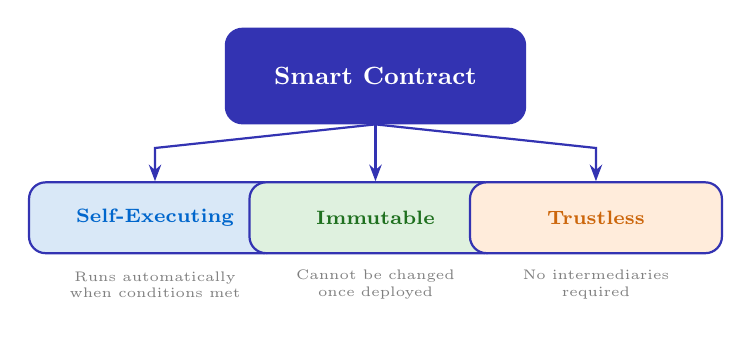
\begin{tikzpicture}[
  box/.style={rectangle, rounded corners=6pt, draw=mlpurple, thick,
              minimum width=3.8cm, minimum height=1.2cm,
              font=\small\bfseries, align=center},
  arr/.style={-{Stealth[length=6pt]}, thick, draw=mlpurple}
]
% Core definition
\node[box, fill=mlpurple, text=white] (sc) at (0,0) {Smart Contract};

% Properties
\node[box, fill=mlblue!15, text=mlblue, minimum width=3.2cm, minimum height=0.9cm, font=\scriptsize\bfseries]
  (self) at (-2.8,-1.8) {Self-Executing};
\node[box, fill=mlgreen!15, text=mlgreen!70!black, minimum width=3.2cm, minimum height=0.9cm, font=\scriptsize\bfseries]
  (imm) at (0,-1.8) {Immutable};
\node[box, fill=mlorange!15, text=mlorange!80!black, minimum width=3.2cm, minimum height=0.9cm, font=\scriptsize\bfseries]
  (trust) at (2.8,-1.8) {Trustless};

\draw[arr] (sc.south) -- ++(-2.8,-0.3) -- (self.north);
\draw[arr] (sc.south) -- (imm.north);
\draw[arr] (sc.south) -- ++(2.8,-0.3) -- (trust.north);

% Descriptors
\node[font=\tiny, text=mlgray, align=center, text width=3cm] at (-2.8,-2.65)
  {Runs automatically\\when conditions met};
\node[font=\tiny, text=mlgray, align=center, text width=3cm] at (0,-2.65)
  {Cannot be changed\\once deployed};
\node[font=\tiny, text=mlgray, align=center, text width=3cm] at (2.8,-2.65)
  {No intermediaries\\required};
\end{tikzpicture}
\end{center}
\end{column}
\begin{column}{0.43\textwidth}
\vspace{4mm}
\begin{block}{Definition}
\small A \textbf{smart contract} is a program stored on a blockchain that automatically executes when predetermined conditions are met---no middlemen, no delays, no trust required.
\end{block}
\vspace{3mm}
\begin{block}{Nick Szabo (1996)}
\small\itshape ``A smart contract is a set of promises, specified in digital form, including protocols within which the parties perform on these promises.''
\end{block}
\end{column}
\end{columns}
\bottomnote{Nick Szabo coined the term ``smart contract'' in 1994, long before Ethereum made them practical on a global scale.}
\end{frame}

% Frame 3: The Vending Machine Analogy
\begin{frame}{The Vending Machine Analogy}
\vspace{2mm}
\begin{center}
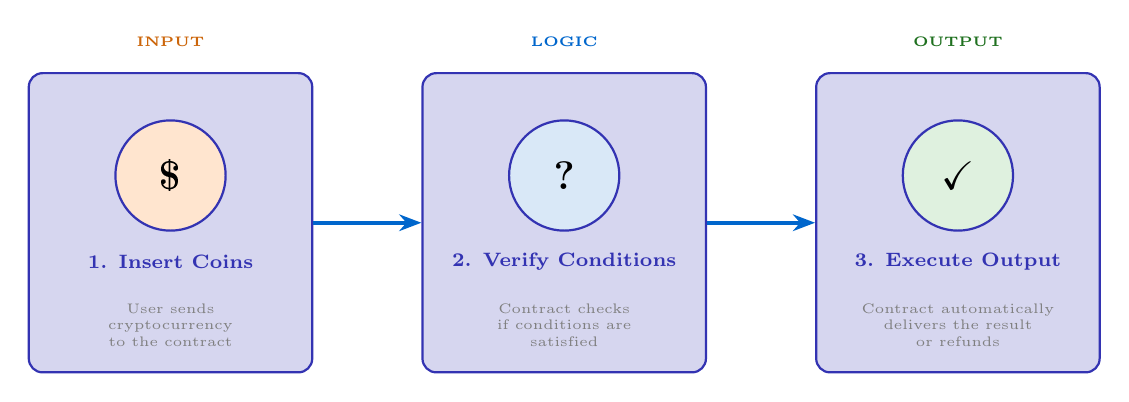
\begin{tikzpicture}[
  panel/.style={rectangle, rounded corners=5pt, draw=mlpurple, thick,
                minimum width=3.6cm, minimum height=3.8cm, fill=mllavender4,
                font=\small, align=center},
  icon/.style={circle, draw=mlpurple, thick, minimum size=1.4cm,
               font=\Large, align=center},
  lbl/.style={font=\scriptsize\bfseries, text=mlpurple},
  sub/.style={font=\tiny, text=mlgray, align=center, text width=3.2cm},
  arr/.style={-{Stealth[length=8pt]}, ultra thick, draw=mlblue}
]
% Panel 1: Insert Coins
\node[panel] (p1) at (0,0) {};
\node[icon, fill=mlorange!20] at (0,0.6) {\textbf{\$}};
\node[lbl] at (0,-0.5) {1. Insert Coins};
\node[sub] at (0,-1.3) {User sends\\cryptocurrency\\to the contract};

% Panel 2: Check Amount
\node[panel] (p2) at (5,0) {};
\node[icon, fill=mlblue!15] at (5,0.6) {\textbf{?}};
\node[lbl] at (5,-0.5) {2. Verify Conditions};
\node[sub] at (5,-1.3) {Contract checks\\if conditions are\\satisfied};

% Panel 3: Dispense
\node[panel] (p3) at (10,0) {};
\node[icon, fill=mlgreen!15] at (10,0.6) {\checkmark};
\node[lbl] at (10,-0.5) {3. Execute Output};
\node[sub] at (10,-1.3) {Contract automatically\\delivers the result\\or refunds};

% Arrows between panels
\draw[arr] (p1.east) -- (p2.west);
\draw[arr] (p2.east) -- (p3.west);

% Labels above
\node[font=\tiny, text=mlorange!80!black] at (0,2.3) {\textbf{INPUT}};
\node[font=\tiny, text=mlblue] at (5,2.3) {\textbf{LOGIC}};
\node[font=\tiny, text=mlgreen!70!black] at (10,2.3) {\textbf{OUTPUT}};
\end{tikzpicture}
\end{center}
\bottomnote{Nick Szabo used the vending machine as the simplest example of a ``smart contract'': deterministic rules, no negotiation, automatic execution.}
\end{frame}

% Frame 4: Smart Contracts vs Traditional Contracts
\begin{frame}{Smart Contracts vs Traditional Contracts}
\vspace{2mm}
\begin{center}
\renewcommand{\arraystretch}{1.5}
\setlength{\tabcolsep}{6pt}
\begin{tabular}{@{}p{3.0cm}p{4.8cm}p{4.8cm}@{}}
\toprule
\textbf{\color{mlpurple}Feature} & \textbf{\color{mlblue}Traditional Contract} & \textbf{\color{mlgreen!70!black}Smart Contract} \\
\midrule
\textbf{Execution} & Manual enforcement by parties or courts & Automatic, self-executing code \\
\textbf{Intermediaries} & Lawyers, banks, notaries & None required \\
\textbf{Speed} & Days to weeks for settlement & Seconds to minutes \\
\textbf{Cost} & High fees for legal and processing & Gas fees only (often \$0.01--\$50) \\
\textbf{Transparency} & Private, restricted access & Public, auditable on-chain \\
\textbf{Modification} & Amendments possible & Immutable once deployed \\
\textbf{Jurisdiction} & Bound by national laws & Borderless, code-is-law \\
\textbf{Dispute Resolution} & Courts and arbitration & On-chain logic or DAO governance \\
\bottomrule
\end{tabular}
\end{center}
\bottomnote{Smart contracts eliminate intermediaries and automate enforcement, but trade flexibility and legal recourse for determinism and speed.}
\end{frame}

% Frame 5: Key Platforms
\begin{frame}{Key Smart Contract Platforms}
\vspace{2mm}
\begin{center}
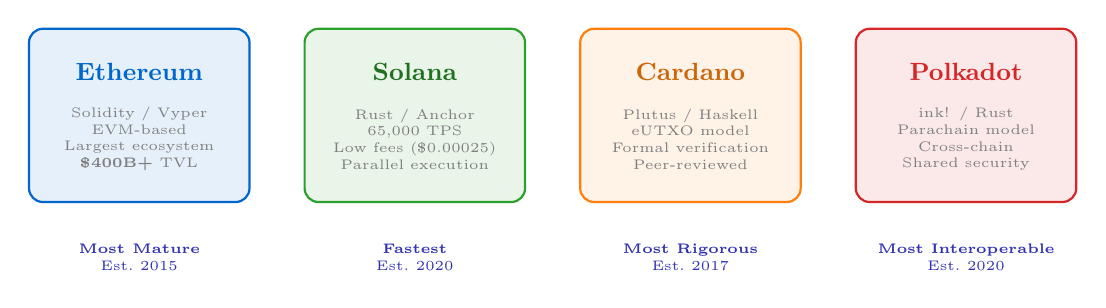
\begin{tikzpicture}[
  pbox/.style={rectangle, rounded corners=5pt, draw=#1, thick, fill=#1!10,
               minimum width=2.8cm, minimum height=2.2cm, align=center},
  ttl/.style={font=\small\bfseries, text=#1},
  det/.style={font=\tiny, text=mlgray, align=center, text width=2.6cm}
]
% Ethereum
\node[pbox=mlblue] (eth) at (0,0) {};
\node[ttl=mlblue] at (0,0.55) {Ethereum};
\node[det] at (0,-0.3) {Solidity / Vyper\\EVM-based\\Largest ecosystem\\\textbf{\$400B+} TVL};

% Solana
\node[pbox=mlgreen] (sol) at (3.5,0) {};
\node[ttl=mlgreen!70!black] at (3.5,0.55) {Solana};
\node[det] at (3.5,-0.3) {Rust / Anchor\\65,000 TPS\\Low fees (\$0.00025)\\Parallel execution};

% Cardano
\node[pbox=mlorange] (car) at (7.0,0) {};
\node[ttl=mlorange!80!black] at (7.0,0.55) {Cardano};
\node[det] at (7.0,-0.3) {Plutus / Haskell\\eUTXO model\\Formal verification\\Peer-reviewed};

% Polkadot
\node[pbox=mlred] (dot) at (10.5,0) {};
\node[ttl=mlred] at (10.5,0.55) {Polkadot};
\node[det] at (10.5,-0.3) {ink! / Rust\\Parachain model\\Cross-chain\\Shared security};

% Comparison bar below
\node[font=\tiny, text=mlpurple, align=center] at (0,-1.8) {\textbf{Most Mature}\\Est.\ 2015};
\node[font=\tiny, text=mlpurple, align=center] at (3.5,-1.8) {\textbf{Fastest}\\Est.\ 2020};
\node[font=\tiny, text=mlpurple, align=center] at (7.0,-1.8) {\textbf{Most Rigorous}\\Est.\ 2017};
\node[font=\tiny, text=mlpurple, align=center] at (10.5,-1.8) {\textbf{Most Interoperable}\\Est.\ 2020};
\end{tikzpicture}
\end{center}
\bottomnote{Ethereum dominates smart contract adoption, but Solana, Cardano, and Polkadot offer distinct trade-offs in speed, rigor, and interoperability.}
\end{frame}

% Frame 6: Real-World Applications
\begin{frame}{Real-World Applications}
\vspace{2mm}
\begin{center}
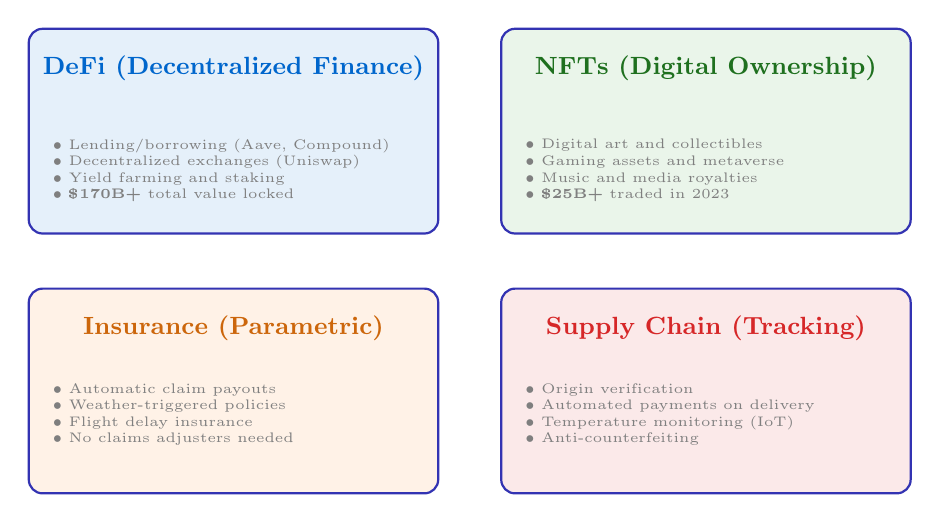
\begin{tikzpicture}[
  qbox/.style={rectangle, rounded corners=5pt, draw=mlpurple, thick,
               minimum width=5.2cm, minimum height=2.6cm, align=center, fill=#1},
  qlbl/.style={font=\small\bfseries, text=#1},
  qdet/.style={font=\tiny, text=mlgray, align=left, text width=4.6cm}
]
% Top-left: DeFi
\node[qbox=mlblue!10] (defi) at (-3.0,1.7) {};
\node[qlbl=mlblue] at (-3.0,2.5) {DeFi (Decentralized Finance)};
\node[qdet] at (-3.0,1.2) {
  $\bullet$ Lending/borrowing (Aave, Compound)\\
  $\bullet$ Decentralized exchanges (Uniswap)\\
  $\bullet$ Yield farming and staking\\
  $\bullet$ \textbf{\$170B+} total value locked
};

% Top-right: NFTs
\node[qbox=mlgreen!10] (nft) at (3.0,1.7) {};
\node[qlbl=mlgreen!70!black] at (3.0,2.5) {NFTs (Digital Ownership)};
\node[qdet] at (3.0,1.2) {
  $\bullet$ Digital art and collectibles\\
  $\bullet$ Gaming assets and metaverse\\
  $\bullet$ Music and media royalties\\
  $\bullet$ \textbf{\$25B+} traded in 2023
};

% Bottom-left: Insurance
\node[qbox=mlorange!10] (ins) at (-3.0,-1.6) {};
\node[qlbl=mlorange!80!black] at (-3.0,-0.8) {Insurance (Parametric)};
\node[qdet] at (-3.0,-1.9) {
  $\bullet$ Automatic claim payouts\\
  $\bullet$ Weather-triggered policies\\
  $\bullet$ Flight delay insurance\\
  $\bullet$ No claims adjusters needed
};

% Bottom-right: Supply Chain
\node[qbox=mlred!10] (sc) at (3.0,-1.6) {};
\node[qlbl=mlred] at (3.0,-0.8) {Supply Chain (Tracking)};
\node[qdet] at (3.0,-1.9) {
  $\bullet$ Origin verification\\
  $\bullet$ Automated payments on delivery\\
  $\bullet$ Temperature monitoring (IoT)\\
  $\bullet$ Anti-counterfeiting
};
\end{tikzpicture}
\end{center}
\bottomnote{Smart contracts power applications from billion-dollar DeFi protocols to parametric insurance that pays out automatically when conditions are met.}
\end{frame}

% Frame 7: How They Work Simplified
\begin{frame}{How Smart Contracts Work --- Simplified}
\vspace{2mm}
\begin{center}
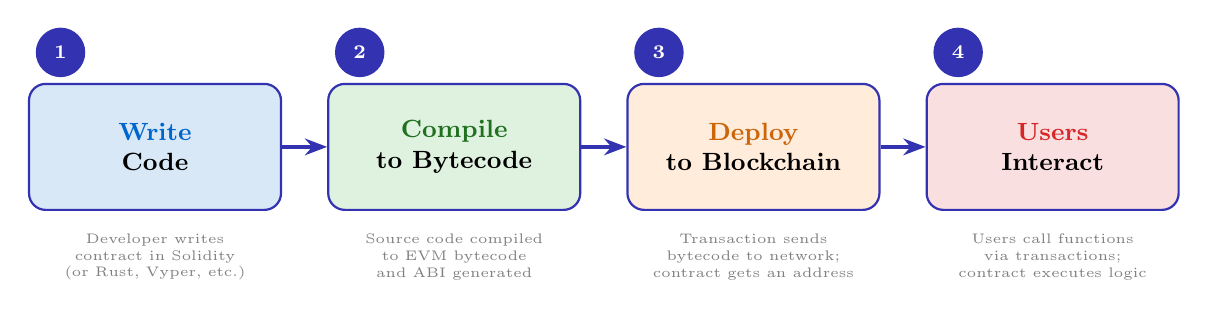
\begin{tikzpicture}[
  step/.style={rectangle, rounded corners=6pt, draw=mlpurple, thick,
               minimum width=3.2cm, minimum height=1.6cm,
               font=\small\bfseries, align=center, fill=#1},
  substep/.style={font=\tiny, text=mlgray, align=center, text width=3.0cm},
  arr/.style={-{Stealth[length=8pt]}, ultra thick, draw=mlpurple},
  num/.style={circle, draw=mlpurple, thick, fill=mlpurple, text=white,
              font=\scriptsize\bfseries, minimum size=0.6cm}
]
% Step 1: Write
\node[step=mlblue!15] (write) at (0,0) {\color{mlblue}Write\\Code};
\node[num] at (-1.2,1.2) {1};
\node[substep] at (0,-1.4) {Developer writes\\contract in Solidity\\(or Rust, Vyper, etc.)};

% Step 2: Compile
\node[step=mlgreen!15] (compile) at (3.8,0) {\color{mlgreen!70!black}Compile\\to Bytecode};
\node[num] at (2.6,1.2) {2};
\node[substep] at (3.8,-1.4) {Source code compiled\\to EVM bytecode\\and ABI generated};

% Step 3: Deploy
\node[step=mlorange!15] (deploy) at (7.6,0) {\color{mlorange!80!black}Deploy\\to Blockchain};
\node[num] at (6.4,1.2) {3};
\node[substep] at (7.6,-1.4) {Transaction sends\\bytecode to network;\\contract gets an address};

% Step 4: Interact
\node[step=mlred!15] (interact) at (11.4,0) {\color{mlred}Users\\Interact};
\node[num] at (10.2,1.2) {4};
\node[substep] at (11.4,-1.4) {Users call functions\\via transactions;\\contract executes logic};

% Arrows
\draw[arr] (write.east) -- (compile.west);
\draw[arr] (compile.east) -- (deploy.west);
\draw[arr] (deploy.east) -- (interact.west);
\end{tikzpicture}
\end{center}
\bottomnote{The lifecycle: write human-readable code, compile to machine bytecode, deploy via a transaction, then anyone can interact with the contract at its address.}
\end{frame}

% Frame 8: Security and Limitations
\begin{frame}{Security Considerations and Limitations}
\vspace{2mm}
\begin{center}
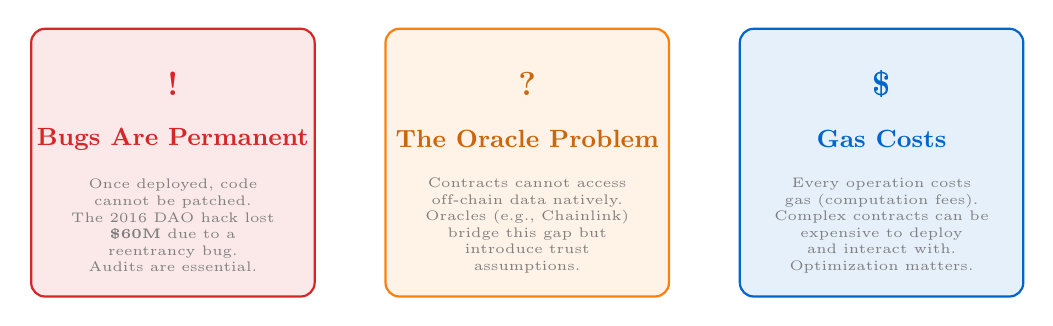
\begin{tikzpicture}[
  card/.style={rectangle, rounded corners=5pt, draw=#1, thick, fill=#1!10,
               minimum width=3.6cm, minimum height=3.4cm, align=center},
  ctitle/.style={font=\small\bfseries, text=#1},
  cdesc/.style={font=\tiny, text=mlgray, align=center, text width=3.2cm},
  warn/.style={font=\large\bfseries, text=#1}
]
% Card 1: Bugs Are Permanent
\node[card=mlred] (bug) at (0,0) {};
\node[warn=mlred] at (0,1.0) {!};
\node[ctitle=mlred] at (0,0.3) {Bugs Are Permanent};
\node[cdesc] at (0,-0.8) {Once deployed, code\\cannot be patched.\\The 2016 DAO hack lost\\\textbf{\$60M} due to a\\reentrancy bug.\\Audits are essential.};

% Card 2: Oracle Problem
\node[card=mlorange] (oracle) at (4.5,0) {};
\node[warn=mlorange!80!black] at (4.5,1.0) {?};
\node[ctitle=mlorange!80!black] at (4.5,0.3) {The Oracle Problem};
\node[cdesc] at (4.5,-0.8) {Contracts cannot access\\off-chain data natively.\\Oracles (e.g., Chainlink)\\bridge this gap but\\introduce trust\\assumptions.};

% Card 3: Gas Costs
\node[card=mlblue] (gas) at (9.0,0) {};
\node[warn=mlblue] at (9.0,1.0) {\$};
\node[ctitle=mlblue] at (9.0,0.3) {Gas Costs};
\node[cdesc] at (9.0,-0.8) {Every operation costs\\gas (computation fees).\\Complex contracts can be\\expensive to deploy\\and interact with.\\Optimization matters.};
\end{tikzpicture}
\end{center}
\bottomnote{Smart contract security is critical: immutability means bugs are permanent, oracles introduce external trust, and gas costs constrain complexity.}
\end{frame}

% Frame 9: Why This Matters
\begin{frame}{Why Smart Contracts Matter}
\begin{columns}[T]
\begin{column}{0.48\textwidth}
\vspace{2mm}
\begin{block}{Key Statistics}
\begin{itemize}\setlength\itemsep{5pt}
  \item[\small$\checkmark$] \small \textbf{\$170B+} locked in DeFi smart contracts
  \item[\small$\checkmark$] \small \textbf{50M+} unique smart contract addresses on Ethereum
  \item[\small$\checkmark$] \small \textbf{4M+} smart contracts deployed in 2024 alone
  \item[\small$\checkmark$] \small \textbf{\$3B+} annual spending on smart contract audits
  \item[\small$\checkmark$] \small \textbf{70\%+} of blockchain transactions involve smart contracts
\end{itemize}
\end{block}
\end{column}
\begin{column}{0.48\textwidth}
\vspace{2mm}
\begin{block}{Impact Areas}
\begin{itemize}\setlength\itemsep{5pt}
  \item[\small$\checkmark$] \small \textbf{Finance:} Eliminating intermediaries in lending, trading, insurance
  \item[\small$\checkmark$] \small \textbf{Governance:} DAOs managing billions in community treasuries
  \item[\small$\checkmark$] \small \textbf{Legal:} Self-enforcing agreements reducing court dependency
  \item[\small$\checkmark$] \small \textbf{Identity:} Decentralized identity and credential verification
  \item[\small$\checkmark$] \small \textbf{Real Estate:} Tokenized property and automated escrow
\end{itemize}
\end{block}
\end{column}
\end{columns}
\bottomnote{Smart contracts are reshaping industries by automating trust, reducing costs, and enabling programmable agreements at global scale.}
\end{frame}

% Frame 10: Coming Up: The Full Lecture
\begin{frame}{Coming Up: The Full Lecture}
\vspace{2mm}
\begin{center}
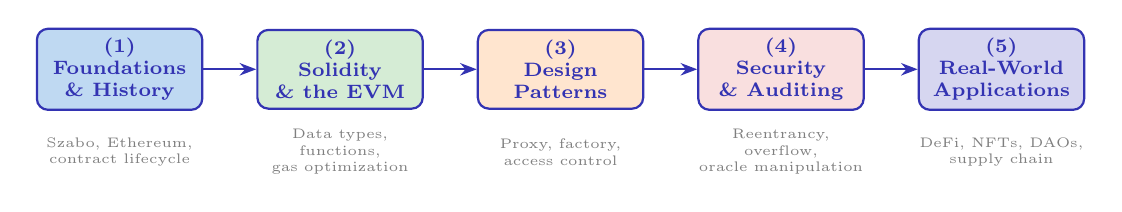
\begin{tikzpicture}[
  secbox/.style={rectangle, rounded corners=4pt, draw=mlpurple, thick,
                 minimum width=2.1cm, minimum height=1.0cm,
                 fill=mllavender3, font=\scriptsize\bfseries,
                 align=center, text=mlpurple},
  conn/.style={-{Stealth[length=6pt]}, thick, draw=mlpurple}
]
\node[secbox, fill=mlblue!25]    (s1) at (0,0)    {(1)\\Foundations\\\& History};
\node[secbox, fill=mlgreen!20]   (s2) at (2.8,0)  {(2)\\Solidity\\\& the EVM};
\node[secbox, fill=mlorange!20]  (s3) at (5.6,0)  {(3)\\Design\\Patterns};
\node[secbox, fill=mlred!15]     (s4) at (8.4,0)  {(4)\\Security\\\& Auditing};
\node[secbox, fill=mlpurple!20]  (s5) at (11.2,0) {(5)\\Real-World\\Applications};

\draw[conn] (s1) -- (s2);
\draw[conn] (s2) -- (s3);
\draw[conn] (s3) -- (s4);
\draw[conn] (s4) -- (s5);

\node[font=\tiny, text=mlgray, align=center, text width=2.1cm] at (0,-1.05)
  {Szabo, Ethereum,\\contract lifecycle};
\node[font=\tiny, text=mlgray, align=center, text width=2.1cm] at (2.8,-1.05)
  {Data types, functions,\\gas optimization};
\node[font=\tiny, text=mlgray, align=center, text width=2.1cm] at (5.6,-1.05)
  {Proxy, factory,\\access control};
\node[font=\tiny, text=mlgray, align=center, text width=2.1cm] at (8.4,-1.05)
  {Reentrancy, overflow,\\oracle manipulation};
\node[font=\tiny, text=mlgray, align=center, text width=2.1cm] at (11.2,-1.05)
  {DeFi, NFTs, DAOs,\\supply chain};
\end{tikzpicture}
\end{center}
\vspace{4mm}
\begin{columns}[T]
\begin{column}{0.48\textwidth}
\begin{block}{Prerequisites}
\begin{itemize}\setlength\itemsep{2pt}
  \item[\small$\checkmark$] \small Basic blockchain concepts (blocks, transactions, consensus)
  \item[\small$\checkmark$] \small Familiarity with any programming language
\end{itemize}
\end{block}
\end{column}
\begin{column}{0.48\textwidth}
\begin{block}{Outcomes}
\begin{itemize}\setlength\itemsep{2pt}
  \item[\small$\checkmark$] \small Read and understand Solidity smart contracts
  \item[\small$\checkmark$] \small Identify common vulnerabilities and security patterns
\end{itemize}
\end{block}
\end{column}
\end{columns}
\bottomnote{The full lecture covers smart contracts from historical foundations through Solidity programming to real-world security and deployment patterns.}
\end{frame}

\end{document}
